% !TEX root = SystemTemplate.tex

\chapter{Overview and concept of operations}

This program is a utility for the testing of student software. In version 1, it took a student's program and checks if it conforms to a suite of test cases and presently, in version 2, looks through a directory heirarchy for all student programs and checks it's conformation to test cases. This document is included on the submission in order to facilitate use and maintenance of the utility. It covers the design, implementation, and usage of the provided software.

\section{Scope}
The scope of this document is meant to be comprehensive, giving users and managers the information necessary to use the product.

\section{Purpose}
The purpose of the Auto Tester is to allow batch-grading. Specifically, this program will run input through a student's code and test if the output is what was expected by the instructor or as created by the generator. A summary file will be generated for each run of the program, detailing which tests passed or failed.


\subsection{Compiling}
The students' program will be supplied as source code, so the Auto Tester must compile it using the GNU C compiler.


\subsection{Identifying Test Cases and Inputting}
For each student program is compiled, the Auto Tester uses searched for files labeled as test cases (a .tst extension). Each test file is then used as input for the student program.


\subsection{Checking Output}
The Auto Tester will re-direct the programs output and evaluate it against the supplied test case. The results of the comparison (pass/fail) are recorded in a log file for each test case encountered.  A final sumary of performance is printed to a final log after all programs have been executed


\section{Systems Goals}
The goal of this system is to provide an environment for test-case grading. This is implemented through the use of the Auto Tester executable, a golden program to test generated test files on (located at the directory of execution) and special test files (placed in any sub-directory or the directory of execution).

The system should be accurate in its output matching and able to do many tests very quickly.

\section{System Overview and Diagram}
The Auto Tester is a highly independent system. It takes as input a students source code, several test case files, and outputs the results of the tests. Externally it does not require much components. A gcc compiler is a must on the target system, but other than that the program relies on the filesystem to fetch its test cases.

Internally, the Auto Tester has 3 major components:
\begin{enumerate}
    \item A function that fetches the filenames of each test case found in the programs directories and subdirectories.
    \item A function that opens each input file and runs it through the student program, capturing the output.
    \item A function that takes each test case output and checks it against the expected answer. This records the results in a log file.
\end{enumerate}

These components combine to test the student program with multiple test cases and output valuable information to be used for grading.

\begin{figure}[tbh]
\begin{center}
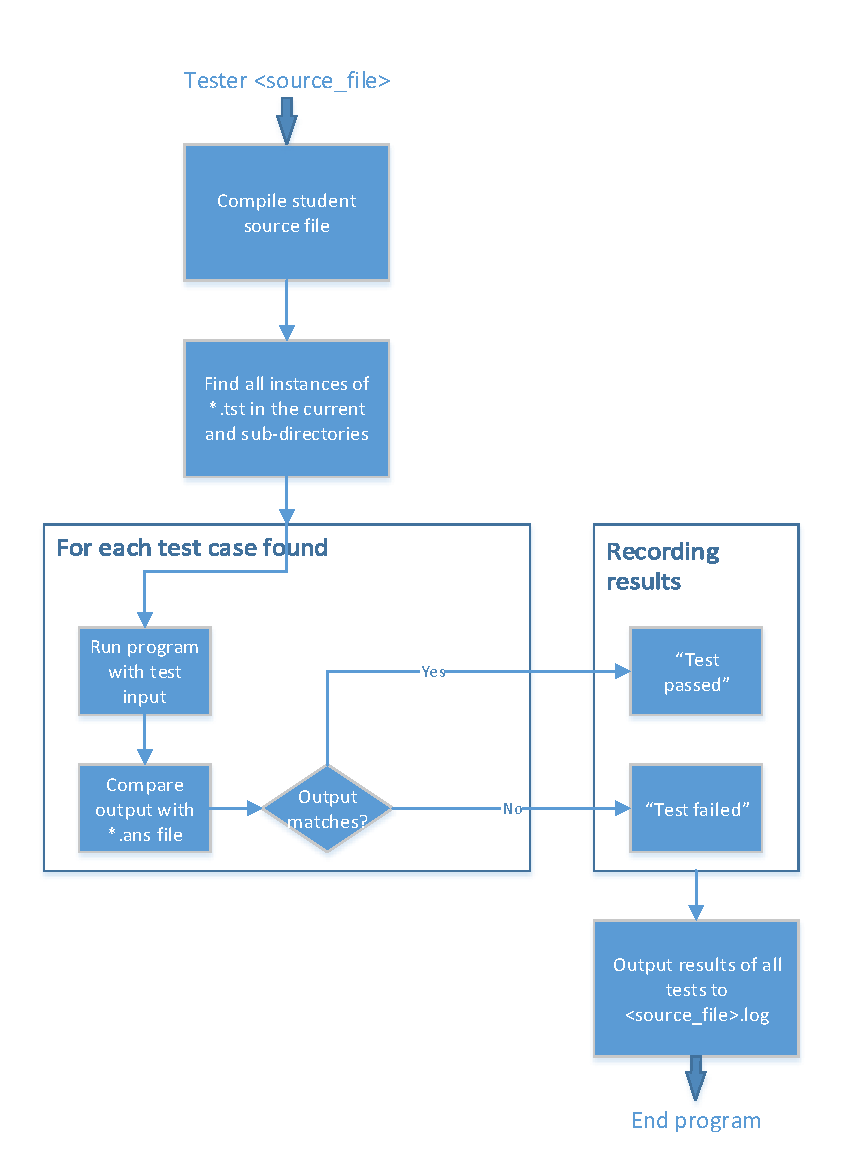
\includegraphics[width=0.60\textwidth]{./Tester}
\end{center}
\caption{The program flow of the Tester \label{systemdiagram}}
\end{figure}

\section{Technologies Overview}
See Table~\ref{somenumbers}. All technology and programs used to develop and run the Auto Tester can be found on any modern GNU\textbackslash Linux distribution.

\begin{table}[tbh]
\begin{center}
\begin{tabular}{|r|l|}
\hline
    GNU C Compiler & For compiling the students program \\ \hline
    GNU find & A command in GNU tools used to search directories \\ \hline
    popen & A function from stdio.h, used to fork a process and supply it with input \\
    \hline
    C++ Template Libraries & Specifically the vector container \\
    \hline
\end{tabular}
\caption{Technologies used in Auto Tester \label{somenumbers}}
\end{center}
\end{table}

